\chapter{Axion Physics and Detection with Resonant Cavities}

This chapter begins by introducing dark matter and how a theoretical particle, the axion, may resolve this long-standing enigma. A brief historical section on particle detectors is presented to provide context for current-generation detector experiments. A discussion of current experiments to detect axions is also given, including various strategies to probe different mass ranges and types of coupling. Finally, a deep dive into the resonant haloscope detector design is provided.

    \section{The Axion} \label{sec:axion}
    
    The $\Lambda$CDM cosmological model~\cite{popoloSmallScaleProblems2017} indicates that approximately 85\% of the universe’s matter consists of dark matter, which may account for deviations observed in galactic rotation curves~\cite{Begeman:1991iy}, gravitational lensing~\cite{Clowe:2006eq}, cosmic microwave background anisotropies~\cite{WMAP:2010qai}, and galaxy cluster collisions~\cite{zwickyRotverschiebungExtragalaktischenNebeln1933}. The matter is called dark because it interacts weakly with light. Particle theorists have proposed many solutions to the dark matter problem. Weakly Interacting Massive Particles (WIMPs) were one of the first dark matter candidates, but these particles have not yet been found at the energies predicted. This suggests that WIMPs might not account for the observed dark matter~\cite{Malik:2012sa, lowetteSupersymmetrySearchesATLAS2012}, so alternative theories have been proposed (Fig.~\ref{fig:DarkMatterContenders})~\cite{rosenbergSearchingDarkHunt2018}.

%and is therefore dark

    A new particle called the axion is gaining traction as the best possible candidate for dark matter, first proposed by Peccei and Quinn (PQ symmetry breaking)~\cite{pecceiMathrmCPConservation1977} in 1977 and Weinberg in 1978~\cite{Weinberg:1978ma}. There may be many axion-like particles (termed the axiverse), some of which naturally arise in fundamental models such as string theory~\cite{Witten:1997sc}. This leads to optimism in the community, since the axion may naturally emerge from a deeper theory, but also pessimism that the axion signal may be further suppressed, given many different axion-like particles.

    %The existence of a vast landscape of axion-like particles—the so-called “axiverse”—emerges naturally in ultraviolet completions such as string theory~\cite{Arvanitaki:2009fg, Acharya:2010zx, Svrcek:2006yi}. This theoretical embedding motivates considerable optimism that (at least one) axion-like particle is realised in nature. At the same time, it gives rise to a more pessimistic perspective: in scenarios with a densely populated axiverse, anthropic selection or dynamical effects typically favour regions of parameter space where the cosmologically observed dark matter relic is composed of axions with smaller decay constants (and hence weaker couplings to Standard Model fields) than in the classic single-axion window. Consequently, detectable signals in laboratory experiments, astrophysical probes, or cosmological observations may be significantly suppressed, rendering detection substantially more challenging.

    Properties of the axion mainly depend on the value of the axion decay constant $f_a$, which is inversely proportional to the axion mass $m_a$~\cite{Weinberg:1978ma}:
    
    \begin{equation}
        m_a \approx  6 \times10^{-5}~\text{eV} \left( \frac{10^{12}~\text{GeV}}{f_a} \right) \,.
        \label{eq:massscaling}
    \end{equation}
    
    \noindent This theory claims that in the early universe, the axion field underwent ``vacuum realignment", which produced cold dark matter with density $\rho_a \propto f_a^2 \theta_{in}^2$, where $\theta_{in}$ is the initial misalignment angle. In the simplest axion model, when $\theta_{in} \sim \mathcal{O}(1)$ and the axion density equals the dark matter density $\rho_a \simeq \rho_{\text{DM}} \approx 0.4$ GeV/cm$^3$, the predicted axion mass is on the order of $10^{-5}$ eV (corresponding to $f_a \sim 10^{12}$ GeV) \cite{Braine:2024nzi}. 
    
    The axion mass has large uncertainties due to the homogenization of the axion field during inflation, topological defects, and the unknown composition of dark matter. Literature has bounded the axion mass to a range of $10^{-13}$ to $10^{-2}$ eV. The lower bound comes from the age of the universe, and the upper bound from accelerator and stellar evolution constraints~\cite{Sikivie:1983ip}. Early experiments searching for the axion yielded null results, as its coupling to ordinary matter was speculated to be too weak for detection~\cite{Sikivie:2020zpn}. As will be discussed in the next section, particle detector sensitivity has improved significantly over time, and the new generation of detectors may be able to detect the weak axion signal.
        
    \begin{figure}
        \centering
        \includegraphics[width=.8\textwidth]{images/intro/DarkMatterContenders.png}
        \caption[Proposed Dark Matter candidates.]{Proposed Dark Matter candidates. By Jen Christiansen; Article by Leslie Rosenberg, Scientific American, January 2018~\cite{rosenbergSearchingDarkHunt2018}.}
        \label{fig:DarkMatterContenders}
    \end{figure}
    
\section{Particle Detectors}

    \subsection{Antiquity to Modern}
        
    \begin{figure}
        \centering
        \includegraphics[width=.2\textwidth]{images/intro/RontgenWifeHand.pdf}
        \caption{Anna Bertha's hand, imaged using Wilhelm Röntgen's X-ray detector in 1895.}
        \label{fig:RontgenWifeHand}
    \end{figure}
    
    The historical context in this section gives perspective on how greatly detectors have improved over the past 130 years. In 1895, Wilhelm Röntgen painted a fluorescent material on a piece of cardboard, creating the world's first particle detector~\cite{glasserWilhelmConradRontgen1993}. This fluorescent material glowed brightly when Wilhelm accelerated electrons into a metal target, producing X-rays that then hit the screen. He asked his wife to put her hand in front of the X-rays, and the first X-ray image was produced (Figure~\ref{fig:RontgenWifeHand}). 

    Radioactivity, the electron, and the structure of the atom were all analyzed using fluorescent detectors. However, a fluorescent screen can only detect where a particle has ended up and provides no information about the particle’s momentum. Shortly after, in the early 1900s, the cloud chamber was invented. This enabled the visualization of particle tracks and momentum estimation, leading to the discovery of new particles such as the positron (Fig.~\ref{fig:positron}), muon, and kaon~\cite{charlesthomsonreeswilsonMethodMakingVisible1911, andersonPositiveElectron1933, andersonCloudChamberObservations1936, rochesterdr.EvidenceExistenceNew1947}.

    \begin{figure}
            \centering
            \includegraphics[width=.5\textwidth]{images/intro/positron.pdf}
            \caption{Cloud chamber track used to prove the existence of the positron in 1932 by Carl Anderson.}
            \label{fig:positron}
    \end{figure}


    %add details to detector numbers
        
    The scientific community has continued to innovate particle detectors, using knowledge from the semiconductor industry to create modern-day scintillators~\cite{greskovichCERAMICSCINTILLATORS1997}. These near-perfect doped-silicon crystals demonstrate significant improvement in sensitivity and detection time. New superconducting thin film technology such as transition edge sensors (TES)~\cite{irwinTransitionEdgeSensors2005} and microwave kinetic induction devices (MKIDs)~\cite{mazinSuperconductingMaterialsMicrowave2021}, have shown orders of magnitude improvement in sensitivity due to their ability to detect small changes in temperature and frequency by taking advantage of the very rapid change of resistance during the transition of a superconductor to the normal state. As will be described later, superconductivity plays a key role in axion detectors. With these new advancements developed through collaborations across many institutions, the community has an unprecedented capability to analyze more data and detect weaker interactions.
    
    A recent example of success with modern detector technology and large-scale collaboration is the Laser Interferometer Gravitational-Wave Observatory (LIGO), which directly detected gravitational waves using interferometers at two sites separated by 3000 km across the United States~\cite{LIGOScientific:2007fwp}. The Deep Underground Neutrino Experiment (DUNE) is another large-scale effort, using a 700-ton container of liquid argon connected to $10^{6}$ scintillators to study neutrino oscillations~\cite{DUNE:2021tad}. Of direct relevance to this dissertation, the Axion Dark Matter eXperiment (ADMX) employs state-of-the-art superconducting quantum sensors (TES and MKIDs) and high-field, large-bore magnets, with plans to integrate superconducting thin-film resonators~\cite{duffyHighResolutionSearch2006, ADMX:2018gho}.
    
    \subsection{Summary of Axion Detection Experiments}
    
    Axions can couple with photons, spins, or gluons, leading to many different types of experiments that probe for axion dark matter. A non-exhaustive list of these experiments include: ADMX~\cite{duffyHighResolutionSearch2006}, investigates axion-photon coupling with a large resonant cavity; QUAX~\cite{FirstQUAXGalactic2020}, exploits spin-precession effects; HAYSTAC~\cite{HAYSTAC:2018rwy}, uses squeezed-state receivers to lower the quantum noise limit; DMRadio~\cite{Silva-Feaver:2016qhh}, optimized for low-mass axions uses lumped-element resonators; MADMAX~\cite{garciaFirstSearchAxion2025}, uses a dielectric haloscopes to scan higher mass ranges; ORGAN~\cite{McAllister:2017lkb}, uses many small cavities; and BREAD~\cite{BREAD:2021tpx}, uses a broadband dish antenna for THz probing. 
    
    This dissertation is closely associated with the ADMX collaboration. The experiments that investigate the photon-axion coupling near GHz frequencies, including ADMX, are given in Fig.~\ref{fig:AxionPhoton_RadioFreqCloseup}.

        \begin{figure}[htb]
        \centering
        \includegraphics[width=.8\textwidth]{images/intro/AxionPhoton_RadioFreqCloseup.pdf}
        \caption{Axion-photon coupling strength vs axion mass for cavity haloscopes~\cite{ciarana.j.ohareAxionLimits2020}.}
        \label{fig:AxionPhoton_RadioFreqCloseup}
    \end{figure}


    As outlined in an extensive review by Sikivie~\cite{Sikivie:2020zpn}, the excluded areas on the plot, denoted by different shaded colored regions, come from a variety of experiments including high-energy astrophysical models, helioscope experiments (axions generated from the sun), heavy axion experiments, and ultralight axion experiments. Sikivie also reviews other coupling schemes, although new and improved modes and corresponding experiments are being proposed every year.  The full theoretical mass range of the QCD-axion experiments is shown in Fig.~\ref{fig:AxionPhoton}.



    
    \begin{figure}[htbp]
        \centering
        \includegraphics[width=.8\textwidth]{images/intro/AxionPhoton.pdf}
        \caption{Axion-photon coupling strength vs axion mass for full axion-photon coupling mass range~\cite{ciarana.j.ohareAxionLimits2020}.}
        \label{fig:AxionPhoton}
    \end{figure}

\section{Resonant Cavity Haloscopes}

    Eight years after the axion was theorized, Pierre Sikivie proposed an experiment to search for the hypothetical axion particles using a resonant cavity haloscope~\cite{Sikivie:1985yu}. This device enables axion detection by combining a strong external magnetic field with a resonant cavity. The Primakoff effect~\cite{primakoffDoubleBetaDecay1959}) converts axions to photons in the magnetic field, and resonant cavities were suggested by Sikivie as the best means to acquire and amplify the photon signal.
    
    The haloscope assumes a specific variety of axions are moving at low velocity, sometimes called ``cold dark matter". This axion is detectable on Earth, since we are immersed in the dark matter halo surrounding our Milky Way galaxy (Fig~\ref{fig:milkwayhalo})~\cite{Battaglia:2005rj, Kafle:2014xfa}. The first axion-probing device was a Cu haloscope cavity made by the ADMX collaboration at the University of Washington~\cite{ADMX:2009iij}. The axion search using a resonant cavity haloscope proceeds through four steps:


\begin{samepage}
   
\begin{enumerate}
    \item The cavity is tuned to the target frequency corresponding to a theoretical axion mass.
    \item The resonance response ($S_{21}$) is measured to verify tuning and extract the loaded quality factor ($Q_L$).
    \item The output signal from the cavity is recorded and integrated to detect possible excess power.
    \item Step to the next frequency and repeat to scan the desired mass range. The desired scan time per frequency is of order 100~s, as a trade-off between detector noise limit and ability to effectively scan across mass ranges over the duration of the experiment.
\end{enumerate}
 
\end{samepage}

    \begin{figure}[htbp]
        \centering
        \includegraphics[width=.5\textwidth]{images/intro/milkywayhalo.jpg}
        \caption[Spherical halo containing dark matter surrounding the visible Milky Way disk.]{Spherical halo containing dark matter surrounding the visible Milky Way disk. Credit: NASA, ESA, and A. Feild}
        \label{fig:milkwayhalo}
    \end{figure}
   
    \subsection{Axion-Photon Conversion Physics}

    When the axion is present within the volume of the resonant cavity, it will couple with the externally applied magnetic field $\textbf{B}_0$~\cite{Sikivie:2020zpn}. This axion-photon coupling is described by the interaction Lagrangian:

    \begin{equation}
         \mathcal{L}_{a\gamma \gamma} = -g_{a\gamma\gamma} \frac{\alpha}{\pi} \frac{1}{f_a} a \textbf{E} \cdot \textbf{B}
         \label{eq:Lagammgamma}
    \end{equation}
    
    \noindent where $\alpha$ is the fine structure constant, $a$ is the axion field operator, $\textbf{E}$ and $\textbf{B}$ are the electromagnetic field operators, and $g_{a\gamma\gamma}$ is a model dependent coupling parameter. In a resonant cavity with an applied magnetic field, this coupling manifests as an induced current density ($\mathbf{J}_{\text{axion}}$) given by:
    
    \begin{equation}
          \mathbf{J}_{\text{axion}} = g_{a\gamma\gamma} \mathbf{E}_{\text{cavity}} \cdot \mathbf{B}_{\text{0}} 
          \label{eq:Jaxion}
    \end{equation}
    
    \noindent where $\mathbf{E}_{\text{cavity}}$ is the resonant cavity's AC electric field and $\mathbf{B}_{\text{0}}$ is the applied DC magnetic field. The axion current density inputs power into the cavity that creates a signal that experiments aim to detect~\cite{Sikivie:2020zpn}.

    \subsubsection{Parallel Field Requirement}


    The axion-photon coupling current (Eq.~\ref{eq:Jaxion}) is maximized when $\mathbf{E}_{\text{cavity}} $ is parallel to $ \mathbf{B}_{\text{0}}$. However, given a single electromagnetic wave, $\mathbf{E}$ and $\mathbf{B}$ are always perpendicular to each other. Therefore, it is not possible to generate parallel electric and magnetic fields from a single source. Instead, two independent field sources are required:

    \noindent ADMX use a cylindrical cavity with its axis aligned with an external magnetic field:
    
    \begin{enumerate}
        \item DC magnetic field ($\mathbf{B}_{\text{0}}$): Generated by an external superconducting solenoid oriented along $z$.
        \item AC electromagnetic field ($\mathbf{E}_{\text{cavity}}$): Generated by a resonant cavity mode where the AC electric field is oriented in the axial-direction, parallel to $\mathbf{B_0}$ (e.g., TM modes).
    \end{enumerate} 

    The coupling between the external magnetic field and the cavity mode is captured in a form factor $C_\alpha$:
        
    \begin{equation}
        C_\alpha = \frac{\left| \int_V \mathbf{E}_{\text{cavity}} \cdot \mathbf{B}_0 \, dV \right|^2}{V \mathbf{B}_0^2 \int_V \epsilon |\mathbf{E}_{\text{cavity}}|^2 \, dV} \, .
        \label{eq:formfactor}
    \end{equation}
    
    \noindent This dimensionless quantity ranges from 0 to 1, with 1 corresponding to maximum dot-product between cavity electric field and external magnetic field ($\mathbf{E}_{\text{cavity}} \parallel \mathbf{B}_0$). For the TM$_{010}$ mode in a cylindrical cavity aligned along the solenoid axis, typical $C_\alpha$ values are $0.4-0.5$ depending on actual cavity  geometry~\cite{Braine:2024nzi}. Shapes optimized for detection are not upright cylinders, because losses at the endcaps reduce the quality factor (discussed in \ref{sec:campbell}). Thus, there is a trade-off between optimizing the cavity shape for high quality factor and optimizing the form factor.

    \subsubsection{Axion Conversion Power}

    The power developed in the cavity when the resonant mode overlaps with the frequency of photons from axion conversion is given by~\cite{ADMX:2018gho}:


    \begin{equation}
        P_{a\gamma\gamma} = g_{a\gamma\gamma}^2 \,  B_{0}^2 \, \frac{\rho_a}{m_a} \, V\,  Q_{L}\, C_{\alpha} \,.\label{eq:FullPower1}  
    \end{equation}

    \noindent where $V$ is the cavity volume, $\rho_a$ is the local axion dark matter density, $m_a$ is the axion mass, and $Q_L$ is the loaded quality factor (measured quality factor). Using typical experimental parameters~\cite{Braine:2024nzi}:

    \begin{equation}
    \begin{split}
        P_{axion} = 1.9 \times 10^{-22} \ \si{W} \left( \frac{V}{136\ \si{l}} \right) \left( \frac{B}{6.8\  \si{T}} \right)^2 \left( \frac{C_{\alpha}}{0.4} \right) \left( \frac{g_{a\gamma\gamma}}{ 0.97}\right)^2 \\ 
        \times \left( \frac{\rho_a}{ 0.45\ \si{GeV} \ \si{cm}^{-3}} \right) \left( \frac{f}{ 650\ \si{MHz}} \right) \left( \frac{Q_{L}}{ 50{,}000} \right).
        \label{eq:FullPower2}  
    \end{split}
    \end{equation}

    \noindent where $g_{a\gamma\gamma}$ is the dimensionless model-dependent coupling constant with values of --0.97 and 0.36 for KSVZ and DFSZ models respectively~\cite{ADMX:2018gho}, and $f$ is the frequency of the cavity mode. The unknown variables are the axion density $\rho_a$, the axion-photon conversion frequency $f$, and the coupling constant $g_{a\gamma\gamma}$.

    \subsection{Resonance Enhancement Mechanism}
    
    \subsubsection{Frequency Matching Requirement}

    The conversion factor between the axion mass and the corresponding photon frequency during the axion-photon conversion in the haloscope cavity is given by the energy-mass equivalence~\cite{alberteinsteinElectrodynmaicsMovingBodies1905, griffithsIntroductionElectrodynamics2023}:
    
    \begin{equation}
        E = m_ac^2 = hf_{\gamma} \,
        \label{eq:masstofrequency}
    \end{equation}
    
    \noindent where $f_{\gamma}$ is the photon frequency when the axion is at rest. With the simplest model where $m_a \sim 10^{-5}$~eV~\cite{Sikivie:2020zpn}, the matching cavity frequency is $f_{\gamma} \approx 2.4$~GHz, when inserting values for fundamental constants $c$ and $h$ in \ref{eq:masstofrequency}. 
    
    When matching photon frequency ($f_{\gamma}$) to cavity resonant frequency $f_0$, dimensions scale inversely with frequency, as shown in Table~\ref{tab:axion_cavity_sizes}, which presents approximate cavity diameters for cylindrical resonators operating in the TM$_{010}$ mode at various axion masses.

    \begin{table}[h]
    \centering
    \caption{Axion mass, corresponding resonant frequency, and cylindrical cavity diameter for axion detection}
    \begin{tabular}{ccc}
    \hline
    Axion Mass [eV] & Frequency [GHz] & Cavity Diameter [mm] \\
    \hline
    $10^{-6}$  & 0.24  & 1300  \\
    $10^{-5}$  & 2.4  & 130  \\
    $10^{-4}$  & 24  & 13  \\
    \hline
    \end{tabular}
    \label{tab:axion_cavity_sizes}
    \end{table}

    At 2.4 GHz, the cavity diameter is approximately 130~mm, which conveniently fits inside the bore of a high-field superconducting MRI magnet~\cite{thulbornChallengesIntegrating94T2006}. At lower masses $m_a<10^{-6}$~eV, the cavity is much too large to fit inside the bore of a high-field magnet, and at higher axion masses $m_a<10^{-4}$~eV, cavity diameters shrink to $13$~mm, presenting challenges for maintaining a large axion-photon cross-section with a shrinking volume. Higher frequencies can be covered by introducing multiple smaller cavities into the magnetic field, which is an active area of exploration~\cite{McAllister:2017lkb, knirckADMXExtendedFrequency2023}. A plot of the QCD-axion parameter space for axion detector experiments in the range of $m_a<10^{-6}$~eV to $m_a<10^{-4}$~eV is given in Fig.~\ref{fig:AxionPhoton_RadioFreqCloseup}. Much of the unexplored space in this figure corresponds to cavities with frequencies between 2 and 20~GHz.

    \subsubsection{Energy Buildup at Resonance}

    The optimal strategy for increasing $\mathbf{E}_{\text{cavity}}$ is to improve the stored energy in the cavity. At resonance, a high-Q cavity accumulates energy over many oscillation cycles before dissipating it, allowing large $\textbf{E}$ field amplitudes to build up even with modest input power. The stored energy in the cavity is given by~\cite{padamseeRFSuperconductivity2009}:

    \begin{equation}
        U = \frac{1}{4} \int_V \left( \epsilon_0 |\mathbf{E}_{\text{AC}}|^2 + \frac{1}{\mu_0} |\mathbf{B}_{\text{AC}}|^2 \right) dV
        \label{eq:stored_energy}
    \end{equation}
    
    \noindent where $\mathbf{E}_{\text{AC}}$ and $\mathbf{B}_{\text{AC}}$ are the oscillating electromagnetic fields of the cavity's resonant mode. Higher stored energy produces larger $\mathbf{E}_{\text{AC}}$ amplitude which, when combined with strong external $\mathbf{B}_0$ for a solenoid magnet, maximizes the axion coupling $\mathbf{E}_{\text{AC}} \cdot \mathbf{B}_0$.

    \subsubsection{Cavity and Axion Bandwidth}

    A cavity at resonant frequency $f_0$ amplifies signals within the bandwidth:

    \begin{equation}
        \Delta f_c = \frac{f_0}{Q_L}\,.
        \label{eq:bandwidth}
    \end{equation}
    
    \noindent For a cavity with $f_0 = 2.4$~GHz and $Q_L = 50{,}000$, the bandwidth is $\Delta f_c \sim 50$~kHz, amplifying signals only within $\pm25$~kHz of resonance.

    The axion signal itself has a finite bandwidth due to the dark matter particles' velocity distribution. Including kinetic energy in the total energy:
        
    \begin{equation}
       E =  m_ac^2 +  \frac{1}{2}m_av^2 = hf_{\text{signal}} \,
        \label{eq:totalEnergy}
    \end{equation}
        
    \noindent Combining with Eq.~\ref{eq:masstofrequency} ($f_{\gamma} = m_ac^2/h$):

    \begin{equation}
        f_{\gamma} \left( 1+ \frac{v^2}{2c^2}\right) = f_{\text{signal}} \,.
        \label{eq:TotalE}
    \end{equation}

    \noindent The velocity spread $\Delta v$ induces a frequency spread. Differentiating Eq.~\ref{eq:TotalE}:

    \begin{equation}
        \frac{\Delta f_{\text{signal}}}{f_{\gamma}} \approx \frac{v \cdot \Delta v}{c^2} \,.
        \label{eq:FSpreadVSpread}
    \end{equation}

    \noindent For QCD axions constituting the galactic dark matter halo, $v \sim 270$~km/s $\approx 10^{-3}c$~\cite{lewinReviewMathematicsNumerical1996, evansRefinementStandardHalo2019}. Virial equilibrium implies $\Delta v \sim v$, giving a signal bandwidth:
    
    \begin{equation}
        \Delta f_{\text{signal}} \sim 10^{-6} \cdot f_{\gamma} \,,
    \end{equation}
    
    \noindent corresponding to an axion quality factor $Q_a \equiv f_{\gamma}/\Delta f_{\text{signal}} \sim 10^6$. This sets the intrinsic width of the axion signal in frequency space. 

    It was previously thought that once the cavity quality factor exceeded the axion quality factor ($Q_L > Q_a$), further increases in cavity quality factor would not improve scan rate. However, \citeauthor{Cervantes:2022gtv}~\cite{Cervantes:2022gtv} found that scan rate remains proportional to $Q_L$ even when $Q_L \gg Q_a$, motivating the pursuit of ultra-high-Q superconducting cavities for axion detection.
    
    \subsection{Quality Factor}\label{sec:QualityCh2}

    The loaded quality factor ($Q_L$) of the cavity is determined by the losses from the cavity walls ($Q_0$) and all other loss mechanisms ($Q_S$):

    \begin{equation}
        \frac{1}{Q_L}= \frac{1}{Q_0} + \frac{1}{Q_s} .  \label{eq:QualityHW} 
    \end{equation}

    \noindent With highly optimized materials (high $Q_0$) and minimizing the impact of other losses (ensuring minimal RF leakage and weak antenna coupling $Q_s>>Q_0$ see App.~\ref{sec:RFCharacterization}), the loaded quality factor $Q_L$ can be maximized. This explains how a better understanding of the materials science of cavity materials can lead to improved quality factor, which is the central thrust of this dissertation. Quality factor can also be calculated using:
        
    \begin{align}
        Q = \frac{G}{R_s} \label{eq:Q0_geometric} \,,
    \end{align}
    
    \noindent where $G$ is the geometric factor (units: $\Omega$) and $R_s$ is the AC surface resistance (units: $\Omega$). 

    \subsubsection{Geometric Factor}
    
    The geometric factor is defined as~\cite{padamseeRFSuperconductivity2009}:
    
    \begin{align}
       G = \frac{\omega_0 \text{~(stored magnetic energy)}}{\text{(power loss per unit } R_s \text{)}} = \frac{2\pi f_0 \mu_0 \int_V |\vec{H}|^2 \, dV}{\int_S |\vec{H}_t|^2 \, dA}  \label{eq:geometric_factor} ,
    \end{align}
   
    \noindent where $f_0$ is the resonant frequency ($2\pi f_0 = \omega_0$), $\mu_0 = 4\pi \times 10^{-7}$~H/m is the permeability of free space, $\textbf{H}$ is the AC magnetic field of the resonant cavity mode in volume $V$, $\textbf{H}_t$ is the tangential AC magnetic field at the cavity surface $S$, and $dV$, $dA$ are internal volume and surface elements of the cavity respectively. 
    
    Note that $G$ is a purely geometric property of the cavity and its resonating mode. $G$ can be analytically solved for simple geometries, but is usually numerically solved using finite element (FEM) eigenfrequency simulation. 

    \subsubsection{Loss Decomposition}

    One can assign geometric factors to different cavity surfaces:

    \begin{equation}
        \frac{1}{G_{\text{total}}} = \frac{1}{G_1} + \frac{1}{G_2} + \cdots + \frac{1}{G_N}
        \label{eq:G_parallel}
    \end{equation}
        
    The total cavity quality factor (Eq.~\ref{eq:QualityHW}) can be expanded using different surfaces:

    \begin{equation}
        \frac{1}{Q_L} = \underbrace{\frac{R_{s,\text{walls}}}{G_{\text{walls}}}}_{\frac{1}{Q_0}} + \underbrace{\left(\frac{R_{s,\text{seams}}}{G_{\text{seams}}} + \frac{R_{s,\text{antenna}}}{G_{\text{antenna}}} + \cdots \right)}_{\frac{1}{Q_S}}
        \label{eq:Q0_decomposed_grouped}
    \end{equation}

    This surface decomposition reveals that $Q_L$ can still be maximized even when the resistance contributions from the seams and antennas are high. This is provided that their geometric factors are large, thereby minimizing their contribution to total losses.
        
    Surface resistance $R_s$ is a material property that depends on the conductor type, temperature, and frequency. For normal conductors, $R_s$ increases with frequency and decreases with temperature as phonon scattering reduces~\cite{ashcroftSolidStatePhysics1976}. For superconductors, $R_s$ depends on the superconducting transition temperature, normal-state resistivity, and applied magnetic field through mechanisms including the Bardeen-Cooper-Schrieffer (BCS) surface resistance~\cite{bardeenTheoryMeissnerEffect1955} and dissipation due to flux motion~\cite{campbellResponsePinnedFlux1969}.
    
    The detailed physics of surface resistance for both normal conductors and superconductors, including behavior in high magnetic fields, will be described in Chapter~\ref{ch:MaterialScience}.

    \subsection{Experimental Scan Strategy}

    The measurement strategy relies on placing an antenna inside the cavity that couples to inner resonant surface. During normal operation, without contributions from decaying axions, a phase-locked loop recycles power leaving the cavity back into the cavity. Excess power from an axion will shift the output phase, which can be extracted as a signal. The phase-shifted power coupled out of the cavity is amplified and spectrum-analyzed, resulting in a measurable signal $\mathcal{O} (10^{-23}$ W)~\cite{ADMX:2018gho}. Figure~\ref{fig:axionsignal} shows a simulated axion signal imposed on real data. If a peak persists after signal averaging, it can be distinguished from noise or environmental interference by four characteristic properties of the axion signal~\cite{Sikivie:2020zpn}:
    
    \begin{enumerate}
        \item Signal must be independent of microwave shielding around the cavity.
        \item Signal cannot be detected by an antenna outside the cavity.
        \item Its central frequency $\omega_\alpha$ exhibits a Lorentzian lineshape with width set by the axion velocity distribution.
        \item The signal power scales as $\mathbf{B}_0^2$ (proportional to squared magnetic field).
    \end{enumerate}

    \begin{figure}[H]
        \centering
        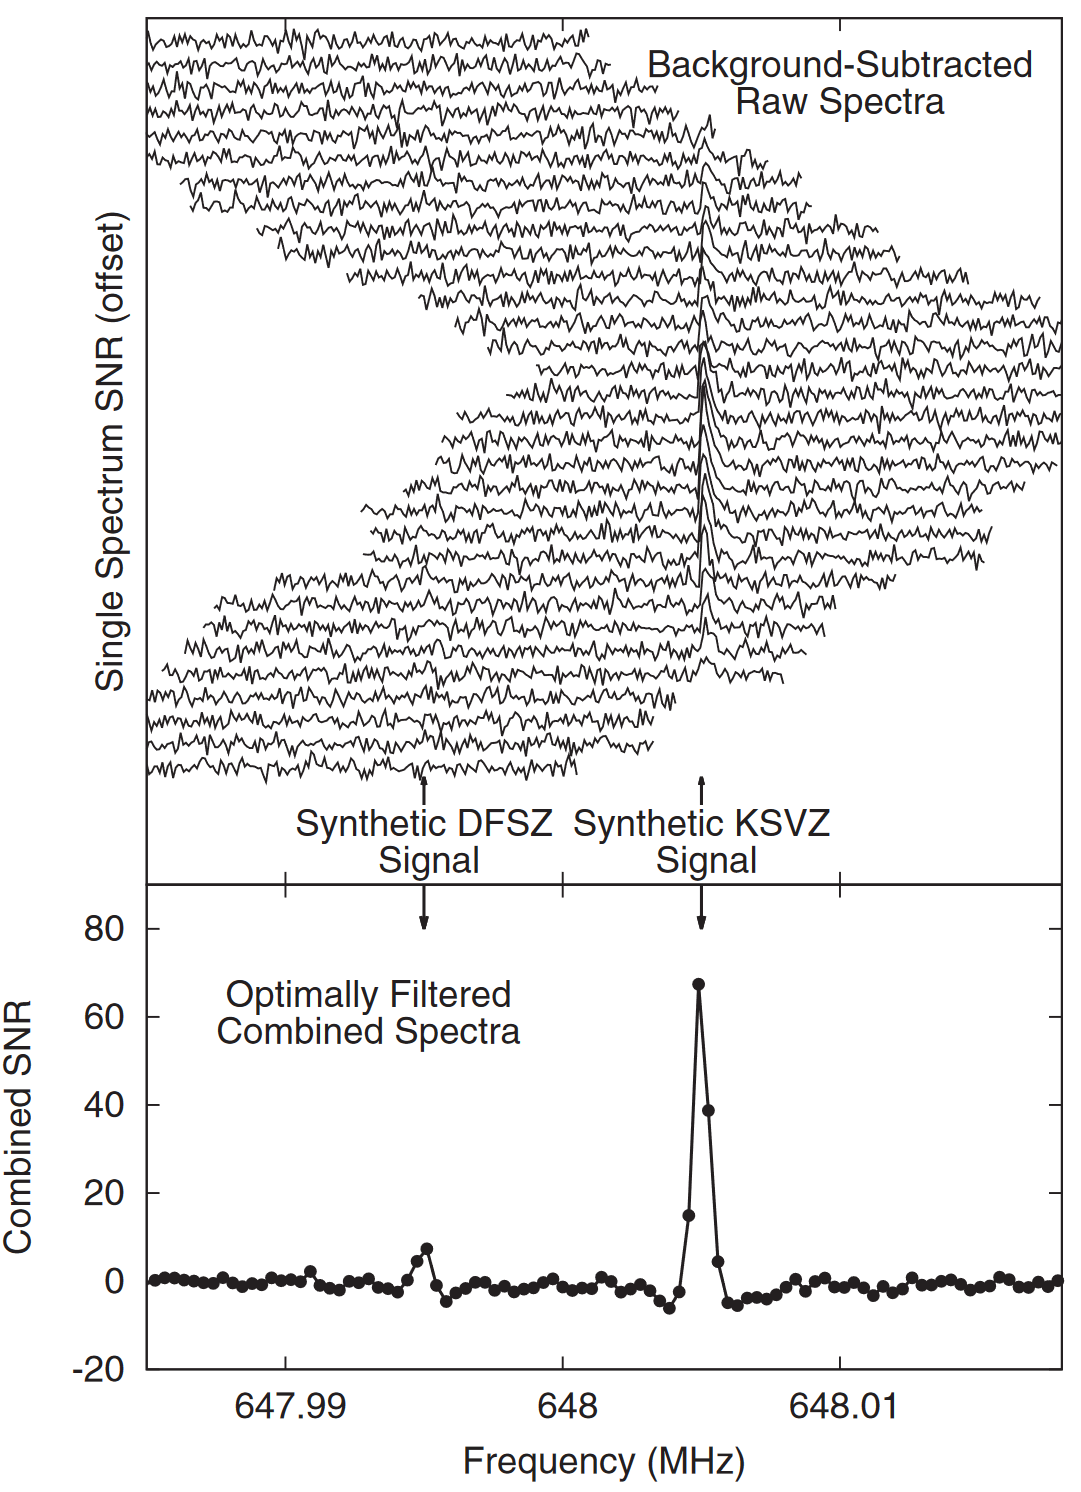
\includegraphics[width=.6\textwidth]{images/intro/syntheticaxion.png}
        \caption[(Upper) Background-subtracted single scans with synthetic axion signals at DFSZ and KSVZ coupling strengths~\cite{Lentz:2017aay}.]{(Upper) Background-subtracted single scans with synthetic axion signals at DFSZ and KSVZ coupling strengths~\cite{Lentz:2017aay}. (Lower) Same data after filtering; both signals become visible~\cite{ADMX:2018gho}.}
        \label{fig:axionsignal}
    \end{figure}
    \FloatBarrier


    \subsubsection{Signal Detection and Discrimination}

    The signal-to-noise ratio is defined as~\cite{Braine:2024nzi}:
    
    \begin{equation}
        SNR = \frac{P_{a\gamma\gamma} }{k_B T_{sys}} \sqrt{\frac{t}{B}}
        \label{eq:signalt:noise}
    \end{equation}
       
    \noindent where $P_{a\gamma\gamma}$ is the axion power deposited into the cavity (Eq.~\ref{eq:FullPower1}), $t$ is the integration time over which the Fourier transform is taken, and $\Delta f$ is the integrated bandwidth of the Fourier transform~\cite{Braine:2024nzi}. ADMX typically uses an SNR of about 3.5, providing a good trade-off between staying on resonance to allow the axion signal to appear above the noise and maintaining an adequate scan rate to cover the frequency space efficiently without prolonging the experiment.



    \subsubsection{Frequency Tuning}

    Scanning to different axion masses with the same cavity requires a movable metal or dielectric rod inserted into the cavity volume~\cite{ADMX:2023rgo}. This tuning rod changes the effective volume seen by the electric field, shifting the resonant frequency by at most $\pm 40\%$ from the base value. Fine-tuning achieves frequency steps smaller than the cavity bandwidth ($\Delta f_c = f_0/Q_L$). For a cavity with $f_0 = 2.4$ GHz and $Q_L = 50{,}000$, the bandwidth is $\Delta f_c \sim 50$ kHz as discussed previously. To cover 2~GHz in one year requires a dwell time per frequency point of approximately $(1/3 \text{ year}) \times 1/Q_L \sim 100$ seconds.

    \subsubsection{Scan Rate Optimization}

    The scan rate, or how quickly the experiment can cover axion parameter space, depends on five experimental parameters~\cite{Braine:2024nzi}:

    \begin{equation}
        \frac{df}{dt} \propto T_{\text{sys}}^{-2} \, \text{SNR}^{-2}  \,   V^{2} \, Q_{L} \, \text{B}^{4} \,.
        \label{eq:scanrate}
    \end{equation}
        
    \noindent Each parameter faces different optimization constraints:
    
    \noindent \text{System Temperature ($T_{\text{sys}}$):} Already minimized using dilution refrigerators (millikelvin operation) combined with quantum-limited amplifiers (Josephson parametric amplifiers and traveling-wave parametric amplifiers).
   
    \noindent \text{Signal-to-Noise Ratio (SNR):} Fixed by statistical detection confidence requirements, cannot be arbitrarily reduced without sacrificing discovery potential.
    
    \noindent \text{Cavity Volume ($V$):} Directly increases signal power (Eq.~\ref{eq:FullPower1}), but diameter determines frequency ($f \propto 1/D$ for TM$_{010}$ mode), so it can not be arbitrarily increased. The cavity can be elongated axially to increase its volume while maintaining a constant resonant frequency, but its length is constrained by the homogeneous field zone in the magnet bore. A multi-cavity array is proposed to increase volume while operating at a higher frequency, $2-4$~GHz (ADMX extended frequency range - EFR~\cite{Braine:2024nzi}).  
    
    \noindent \text{Magnetic Field ($B$):} Despite strong $B^4$ scaling, practical improvements face severe limits. Achieving the same scan-rate improvement when increasing $Q$ from 50,000 to $10^6$ would require increasing the field from 9 T to 19 T, which is beyond the capabilities of any commercially available large-bore superconducting magnet.
    
    \noindent \text{Quality Factor ($Q_L$):} Although scan rate scales only linearly with $Q$, practical improvements span 1--2 orders of magnitude: from $Q \sim 50{,}000$ for high-purity copper cavities to $Q > 10^6$ for optimized superconducting films. This represents the most accessible path to order-of-magnitude improvements in scan rate.
        
    In this context, replacing copper cavities with superconducting thin films offers greater gains than increasing other variables, owing to lower complexity and cost. The development of high-$Q$ superconducting coatings compatible with high magnetic fields is, therefore, critical for accelerating the axion search, which motivated the research presented in this dissertation.

